\documentclass[tikz]{standalone}
\usepackage{pgfplots}
\usepackage{xcolor} % Needed for hex colors
\usetikzlibrary{calc} % For coordinate calculations if needed
\definecolor{markcolor}{HTML}{3c78d8} % Define a custom color
\pgfplotsset{compat=1.18}

\begin{document}
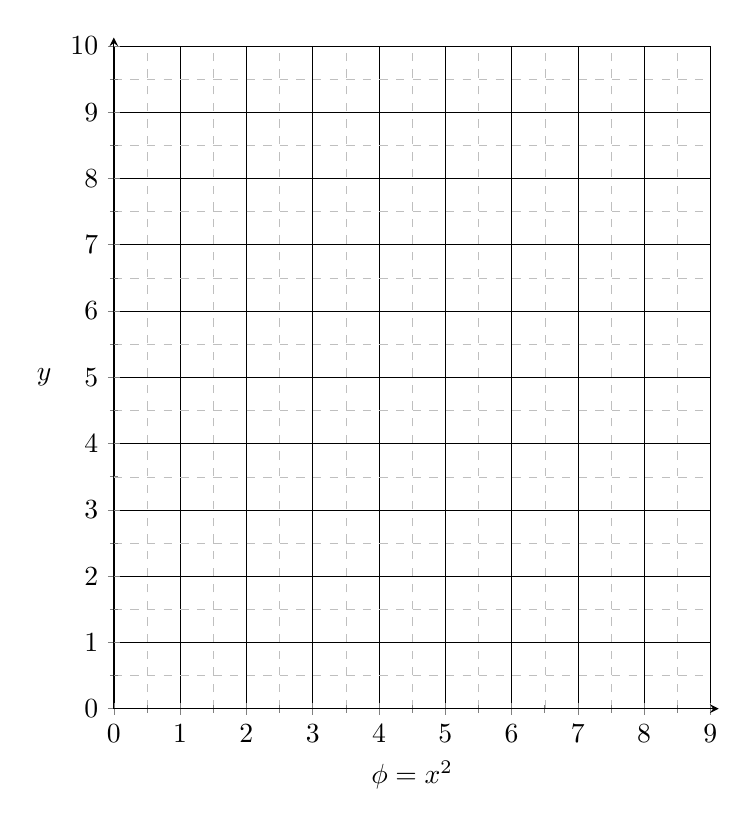
\begin{tikzpicture}
  \begin{axis}[
    axis equal image,
    % Draw only the bottom and left axes with arrow tips:
    axis lines=left,
    x axis line style={->,>=stealth, shorten >=-3pt},
    y axis line style={->,>=stealth, shorten >=-3pt},
    xlabel={\(\phi = x^2\)},
    ylabel={$y$},
    ylabel style={rotate=-90},
    xmin=0, xmax=9,
    ymin=0, ymax=10,
    xtick={0,1,...,9},
    ytick={0,1,...,10},
    minor x tick num=1,
    minor y tick num=1,
    grid=both,
    major grid style={line width=0.2pt,draw=black},
    minor grid style={line width=0.1pt,draw=gray!50,dashed},
    width=10cm,
    height=10cm,
  ]
    % Example marker at (4,6)
    \addplot[only marks, mark=circle*, mark options={scale=1.5, fill=markcolor}] coordinates {(4,6)};
  \end{axis}
\end{tikzpicture}
\end{document}